\documentclass{article}

% if you need to pass options to natbib, use, e.g.:
% \PassOptionsToPackage{numbers, compress}{natbib}
% before loading nips_2017
%
% to avoid loading the natbib package, add option nonatbib:
% \usepackage[nonatbib]{nips_2017}

\usepackage[final]{nips_2017}

% to compile a camera-ready version, add the [final] option, e.g.:
% \usepackage[final]{nips_2017}

\usepackage[utf8]{inputenc} % allow utf-8 input
\usepackage[T1]{fontenc}    % use 8-bit T1 fonts
\usepackage{hyperref}       % hyperlinks
\usepackage{url}            % simple URL typesetting
\usepackage{booktabs}       % professional-quality tables
\usepackage{amsfonts}       % blackboard math symbols
\usepackage{nicefrac}       % compact symbols for 1/2, etc.
\usepackage{microtype}      % microtypography
\usepackage{graphicx}

\title{Midterm Report}

% The \author macro works with any number of authors. There are two
% commands used to separate the names and addresses of multiple
% authors: \And and \AND.
%
% Using \And between authors leaves it to LaTeX to determine where to
% break the lines. Using \AND forces a line break at that point. So,
% if LaTeX puts 3 of 4 authors names on the first line, and the last
% on the second line, try using \AND instead of \And before the third
% author name.

\author{
  Caleb Kaiji Lu\\
  \texttt{caleb.lu@sv.cmu.edu} \\
  %% examples of more authors
  \And
  Nanshu Wang\\
  \texttt{nanshu.wang@sv.cmu.edu} \\
   \And
  Tyler Nuanes\\
  \texttt{tyler.nuanes@sv.cmu.edu} \\
  \And
   Serhan Oztekin\\
  \texttt{serhan.oztekin@sv.cmu.edu} \\
  %% Coauthor \\
  %% Affiliation \\
  %% Address \\
  %% \texttt{email} \\
  %% \AND
  %% Coauthor \\
  %% Affiliation \\
  %% Address \\
  %% \texttt{email} \\
  %% \And
  %% Coauthor \\
  %% Affiliation \\
  %% Address \\
  %% \texttt{email} \\
  %% \And
  %% Coauthor \\
  %% Affiliation \\
  %% Address \\
  %% \texttt{email} \\
}

\begin{document}
% \nipsfinalcopy is no longer used

\maketitle



\section{Project Recap}

There is a strong interest in voice conversion, which is defined as modifying a source speaker's voice to sound as though it were produced by a target speaker. Such technology can have applications ranging from entertainment to speaker recognition. It would be beneficial to games and videos to reproduce the voices of famous actors or actresses for their shows, especially in translating the shows to different languages. It may also help in the grieving process---how many people wish they could hear a loved one's voice one last time after they pass? More sinisterly, such technology could be used by politicians to discredit their enemies by creating false audio in their voice admitting to embarrassing or illegal activities. In our project, we delve into a fundamental algorithm in the field and our work on reproducing and possibly improving it.

\section{Feature Extraction}
Unfortunately for voice conversion technology, speakers have a variety of individual characteristics that affect their speech. Human vocal tract and speaking patterns are highly individualized and humans have evolved a strong ability to discriminate between different speakers [6].  Speaking rate, pitch contour, etc are all various features that help to identify individual speakers. However, some of the most important characteristics of speaker identity are embedded in the statistical distribution of the speech envelope [7]. Based on this concept and previous work, we will focus on voice conversion using the speech envelope as our primary feature.
 
However, human auditory response complicates analysis and reconstruction using only speech envelopes. Specifically, human perception of pitch, or frequency, follows a nonlinear scale. When humans judge whether pitches are equal distances from one another, they select frequencies over larger and larger intervals, starting around 500 Hz. Based on this phenomenon, the Mel scale was developed [2]. A Mel-filter bank can be created to simulate the filtering occurring in the human auditory system with a series of overlapping triangular bandpass filters, centered on the Mel frequencies. 
 
Of additional importance is the actual voiced frequencies. Human speech consists of both ``voiced'' and ``unvoiced'' portions. Voiced sounds are produced by vocal cords, have more amplitude, and can be represented by near-constant frequencies of a particular duration. The maximum voiced frequency tends to be cut off at about 4 kHz. Above this range, there are ``unvoiced'' sounds, which are non-periodic sounds caused by air pressed through a constricted vocal tract. Due to the unperiodic and short-time nature of such events, they tend to have more frequency components and those they have tend to be higher [1]. Studies have shown voiced speech to play a larger role in speaker individuality than unvoiced speech [3], so our conversion will focus on the voiced portions of speech.

Before feeding the features for training, target and source speaker's cepstrums should be aligned using dynamic time warping, a nonlinear method of finding optimal alignment between two time-series data [5]. The algorithm computes the matrix of squared distances between each two points. To discover the warp, it find the path through the matrix that minimizes the total cumulative distances between the two sequences. We use the warp path to generate the aligned features for the source and target.

\section{GMM Model and Conversion function}
Gaussian Mixture Models (GMMs) have been shown to be a reliable choice for voice conversion [3]. A Gaussian Mixture Model represents the data as a weighted sum of Gaussian distributions, each with a characteristic mean and variance. The basic idea is to train GMMs for the joint vector features for source and target spectral features. EM algorithm with Maximum Likelihood Estimation iteratively generates a GMM for the aligned features of the source and target. 

Once we have the GMMs models, the next step is to use GMMs for converting source features to target features. The GMM conversion function deserves special treatment due to its complexity. The primary component of the conversion function is a conditional probability built on the GMM. From the GMM, it is possible to calculate the probability of a target cepstrum given the source speech cepstrum. The paper by Stylianou[3] proposes and compares three different conversion methods: Full, Diagonal, and VQ Conversion. As we know from this course, each class in the GMM model is defined by its parameters: mean and variance. The probability of a target speech class given the source speech vector is obtained from those GMM parameters. Following table shows the comparison of the three conversion functions:

\begin{center}
    \begin{tabular}{ | c | p{6.5cm}  | c | c |}
    \hline
    Conversion & Idea & Performance & computation\\ \hline
    VQ & a weighted sum of each class probability given the source speech vector times the mean target speech vector for the respective class. & poor & simple\\ \hline
    Full & a sum of the VQ conversion and the weighted cross-covariance matrix of the source and target vectors. It is weighted by the inverse covariance times the difference of the source speech vector with the mean for a particular class i. & best & costly\\ \hline
    Diagonal & the cross-covariance of the source and target vectors is set to be diagonal & better than VQ & better than Full\\ \hline
    \end{tabular}
\end{center}   

\section{Algorithm and Implementation}

Based on the complexity of this field and the duration of our project, we chose to implement an algorithm based on a foundational paper in the field. Specifically, Stylianou's foundational work [3], on which more advanced voice conversion technology is based. For instance, given good results from Stylianou's paper, we could look into the paper by Toda et al[4]. The algorithm of Stylianou's paper is essentially as follows:
\begin{enumerate}
\item Create the ``Harmonic + Noise Mode'' model of the speech

\item Calculate the Bark cepstrum

\item Align the target and source speaker's cepstrums

\item Generate the GMM on source and target training data

\item Convert a source cepstrum to the matching target cepstrum using the conversion function
\item Convert the cepstrum back to speech audio:
\begin{enumerate}
\item Convert the cepstrum to the frequency domain.
\item Match the average fundamental frequency to the target.
\item Match the articulation rhythm to the target.
\item Convert the spectrogram back to the time domain.
\end{enumerate}

\item Modify the noise with two fixed filters (one for voiced frames and one for unvoiced frames) and add it to the resulting signal
\end{enumerate}

\begin{figure}
\centering
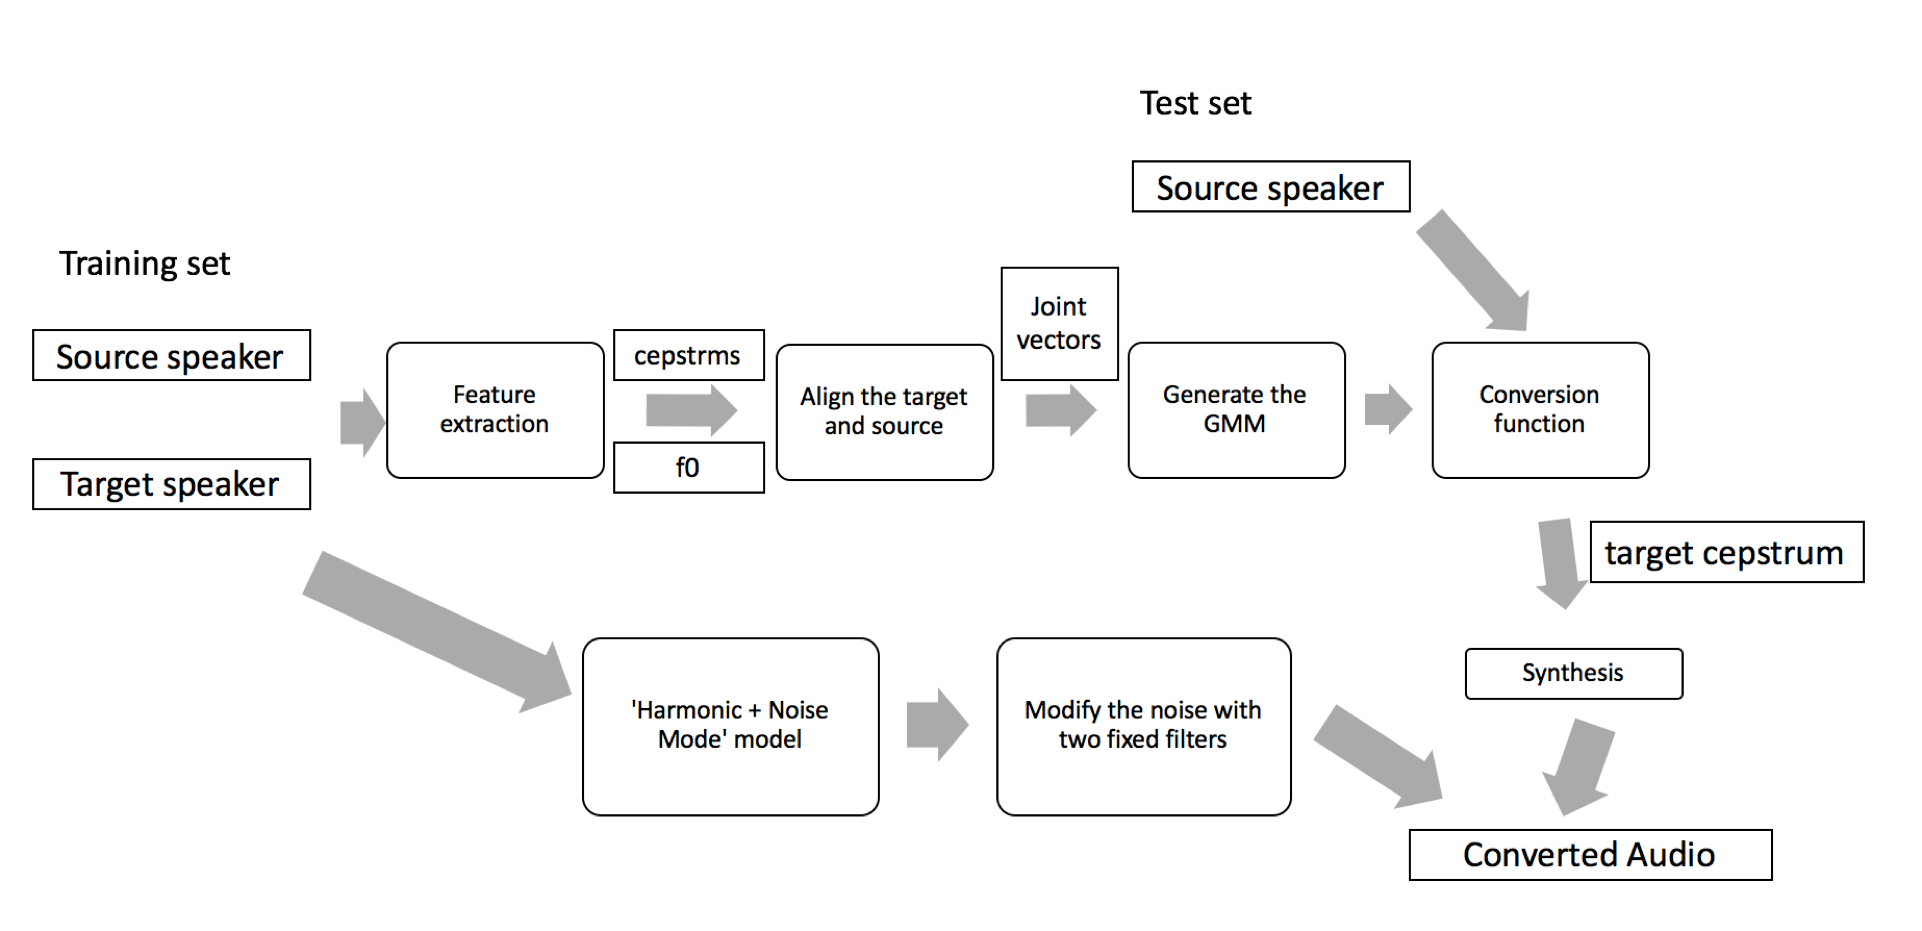
\includegraphics[width=\textwidth]{algorithm.png}
\caption{Voice conversion algorithm workflow}\label{fig:algo}
\end{figure}


So far, we implemented the feature extraction for cepstrums and fundamental frequency, align the source and target feature using dynamic time warping, GMM training and VQ conversion function. We used the dataset from VCC2016[8], which contains 5 source speakers and 5 target speakers. Each speaker utters the same sentence set of 162 sentences. The sampling rate is 16 kHz, and stored in 16-bit format. Due to the complexity of the methods listed above, various python libraries were used for the purpose of this project including dtw, pyworld, pysptk, and sklearn.

\section{Future Work}
  Our code currently performs VQ Conversion. However, Full Conversion is known to provide better results. As this is the case, we will implement the Full Conversion process. In future work, we should also implement improvements on Stylianou's paper, such as those proposed by Toda et al [4]. Once we have caught up with the present state of research, we could focus our efforts on discovering the remaining causes of sub-optimal performance and work to mitigate them.

\section*{References}

\small

[1] Bachu R.G.\ \& Kopparthi S., \ Adapa B., \ Barkana B.D., Separation of Voiced and Unvoiced using Zero crossing rate and Energy of the Speech Signal.  {\it ASEE}. 2008. 
 
[2] Ghosh Debalina,  Depanwita Sarkar Debnath, Saikat Bose, A Comparative Study of Performance of FPGA Based MEL Filter Bank and Bark Filter Bank. {\it International Journal of Artificial Intelligence and Applications}, Vol. 3, No. 3, pp. 37-- 54 (2012). 
 
[3] Stylianou  Yannis,  bOlivier Cappe, and Eric Moulines, Continuous Probabilistic Transform for Voice Conversion. {\it IEEE Transactions on Speech and Audio Processing}, Vol 6, No. 2, pp. 131-142 (1998). 
 
[4] Toda Tomoki, Alan W. Black, Keiichi Tokuda, Voice Conversion Based on Maximum Likelihood Estimation of Spectral Parameter Trajectory. {\it IEEE Transactions on Audio, Speech, and Language Processing}, Vol. 15, No 8, pp 2222--2235 (2007). 
 
[5] Ratanamahatana Chotirat Ann, Eamonn Keogh, Everything you know about Dynamic Time Warping is Wrong. 2004. 
 
[6] Latinus Marianne, Human Voice Perception. {\it Current Biology}, Vol. 21, Iss. 4, (2011). 
 
[7] Reynolds Douglas A., and Richard C. Rose, Robust Text-Independent Speaker Identification Using Gaussian Mixture Speaker Models. {\it IEEE Transactions on Speech and Audio Processing}, Vol. 3, No. 1, pp. 72--83 (1995).

[8] Voice Conversion Challenges 2016. http://vc-challenge.org/vcc2016/summary.html

\end{document}
